%%%%%%%%%%%%%%%%%%%%%%%%%%%%%%%%%%%%%%%%%%%%%%%%%%%%%%%%%%%%%%%%%%%%%%%%%%%%%%%%
% Implementation and algorithm details
%
% - If there are enough content, remove the cache section, it isn't vital to 
%   describe how the cache works.
%%%%%%%%%%%%%%%%%%%%%%%%%%%%%%%%%%%%%%%%%%%%%%%%%%%%%%%%%%%%%%%%%%%%%%%%%%%%%%%%

\chapter{Implementation}
In this section we discuss our implementation. We will briefly discuss our
system design architecture, followed by our modifications to the normal graphics
pipeline. Lastly we will discuss interesting problems that we encountered
and how we attempted to solve these problems. Finally we will discuss performance 
implications.


%%%%%%%%%%%%%%%%%%%%%%%%%%%%%%%%%%%%%%%%%%%%%%%%%%%%%%%%%%%%%%%%%%%%%%%%%%%%%%%


\section{Architecture}
Our prototype implementation is a standard two-tier system: A persistence layer
and a user interface layer. The persistence layer is in charge of database
transactions, cached resources and system state. The user interface layer takes
care of the rendering tasks. 

\begin{figure}
 \centering  
% 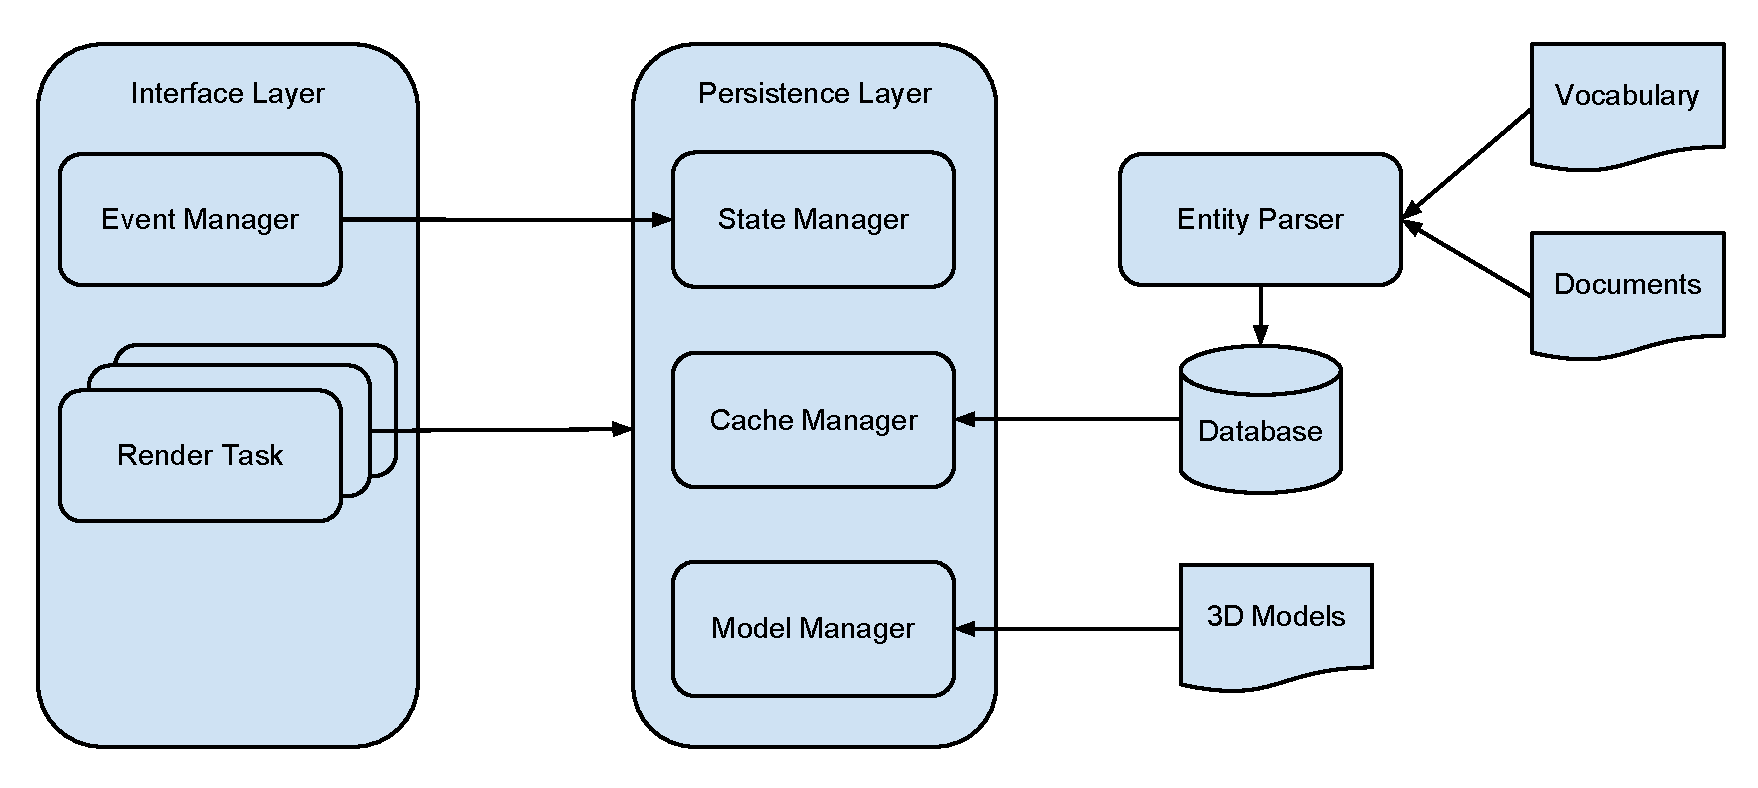
\includegraphics[width=\columnwidth]{Architecture.pdf}
 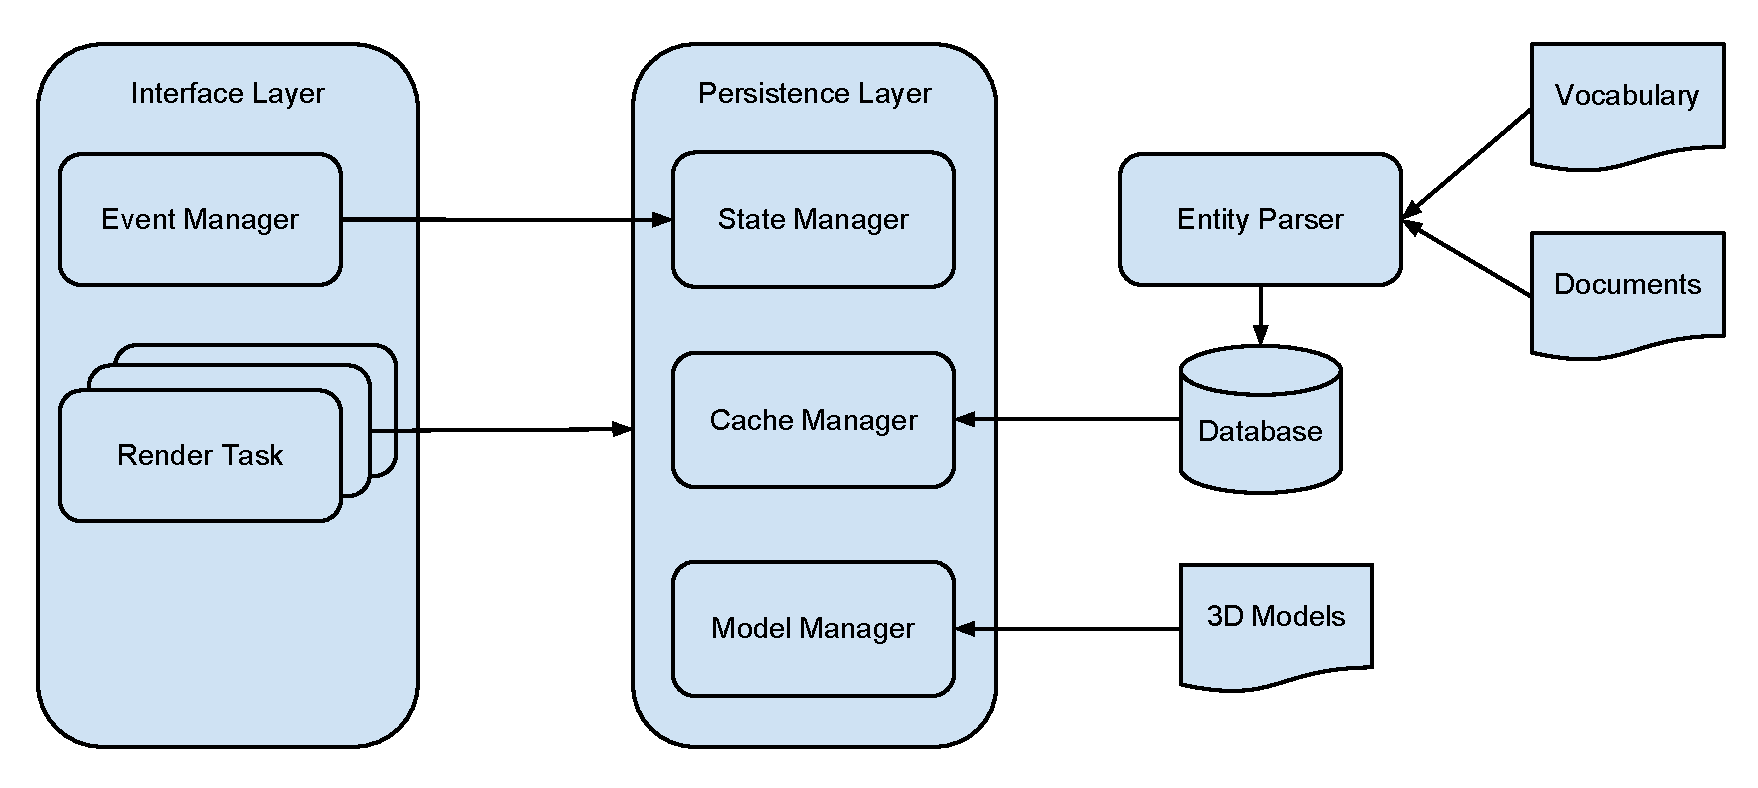
\includegraphics[width=2.5in]{Architecture.pdf} 
 \caption{High level system architecture}
 \label{figure:arch}
\end{figure}


The major components of our system, as well as their functionalities are listed
below: 
\begin{itemize}[noitemsep]
  \item Render Task: Each rendering task is responsible for rendering a
  functional part of the user interface, as well as communicating its states back
  to the persistence layer.
  \item State Manager: It keeps track of all data used for rendering and query
  building.
  \item Model Manager: Holds and manipulate model geometries.
  \item Cache Manager: Stores cache and handles database transactions.
  \item Event Manager: Listens for events, it dispatches changes to the State
  Manager.
\end{itemize}

We should highlight that the Event Manager is not tied to the Render Tasks, and
is only communicating with the State Manager. While this makes dispatching logic
to the UI much more complicated, a separate event handler is easier to
transition to different hardware platforms.


\section{Environment}
The implementation of this prototype is done in the Java programming language.
Graphics are rendered through Java for OpenGL (JOGL) graphics library. A MySQL
database is used to host the text documents as well as their respective document
scores. Our graphics hardware is a NVIDIA Quadro FX video card. The prototype is
designed to run on 1680x1050 screen resolution. 

%%%%%%%%%%%%%%%%%%%%%%%%%%%%%%%%%%%%%%%%%%%%%%%%%%%%%%%%%%%%%%%%%%%%%%%%%%%%%%%
\section{Pipeline Modification}
In order to create our NPR effects and to perform additional semantics on the
visualization, each mesh group are enriched with these additional attributes:

\begin{itemize}[noitemsep]
  \item Adjacent Vertices: Each triangle geometry can have 0 to 3 adjacent
  vertices, these came from neighbouring (connected) triangles. We use these to 
  calculate edges and silhouettes. Where there are no adjacent vertices, we 
  create a placeholder vertices such that it forms a sharp, acute angles with 
  the original triangle.
  \item Centroid: The average XYZ coordinates of all the component�s vertices.
  This is used as inclusion criteria for the lens widget. Other centroid 
  calculation techniques exists, for example ones that takes vertex density and 
  the overall shape into account which gives a better approximation of the 
  logical centre.
  \item Bounding Box: A \threed bounding box (non-axis aligned). We use the
  bounding box to calculate the zone boundaries in screen space.
\end{itemize}
Note we have chosen to use the �triangle soup� approach where each triangle has
distinct vertices. Other methods such as index tables allows neighbouring 
polygons to share vertices which results in better performance and smaller 
footprint, however the cost of this is flexibility and increased complexity for 
handling geometric changes (shared vertices need to be duplicated to avoid 
affecting unaffected polygons). 



%%%%%%%%%%%%%%%%%%%%%%%%%%%%%%%%%%%%%%%%%%%%%%%%%%%%%%%%%%%%%%%%%%%%%%%%%%%%%%%
\section{Algorithms}
During the development of the software prototype, we have encountered several
non-trivial problems. While these issues are not a part of our visualization 
design, they nonetheless impact the overall user experience via the degradation 
of aesthetic and usability of the application. In this section we discuss these 
problems and our proposed solutions.

\subsection{Order Independent Transparency}
We have mentioned briefly that rendering translucent geometries in 3D space can
create artifacts, here we will describe this in greater detail and outline 
possible solutions.
First of all, to create a translucent effect, we need to do two things: 
\begin{itemize} [noitemsep]
  \item Enable Blending: This option allows foreground object to blend with
  background objects.
  \item Disable Depth Testing: This option renders all geometries regardless of
  depth and overlaps.
\end{itemize}
Geometries are typically not sent to the hardware in sorted order, so they are
neither front-to-back nor back-to-front. This is done for a good reason, 
because we don�t typically think of geometries as ordered polygons. Hardware 
supported depth buffer resolves the out-of-order fragments by only only 
selecting the fragment closest to the viewing position. With transparent effect 
in place, fragments are blended together rather than going through the selection 
process. Where the problem arises is that alpha-blending is not commutative, for 
example: red+green+blue does not equal red+blue+green. The result of out-of-order 
blending is that objects that are supposed to be behind can appear to be in front, 
making it difficult for the viewers to judge an object�s depth correctly. 
Naively we can sort the geometries into depth order, or use space partitioning 
structures that forces the geometries to be depth order rendering. However, 
these naive solutions tend to have expensive computation, and are view dependent 
which results in re-computation when the perspective changes. Also, pathological 
cases, for example 3 triangles intersecting each other, cannot be solved with 
partition nor sorting alone.

Recent development in graphics community yield more accurate results, some rely
on re-arrangement of the blending formula to minimize the effects of 
order-dependent terms \cite{Meshkin2007, Bavoil2008}; other use
hardware features to allocate a buffer to emulate sorting, albeit at layers rather than individual
fragments \cite{Myers2007, Bavoil2008, Yang2010}.
In this prototype, we use an implementation of dual-depth-peeling
\cite{Bavoil2008}, which ``peels'' the \threed scene apart layer by layer
into textures, before recomposing these texture into a final texture in depth order. The implication 
of this peeling effect is that it effectively changes the rendering process from
single to multiple passes, a complete rendering will take N/2 passes where N is
the number of geometric layers based on the present viewing position. This 
method yield accurate and eye-pleasing results, while more performance friendly
methods exists, we decided that this was the most reasonable approach because
 the required features are available on most hardware at the time of implementation.


\subsection{Cache and Stabilization}
Due to the size of our data and the diverse variations of queries on the database, 
we have encountered situations where our database does not produce a stable 
performance. We have found with SQL queries alone our query results come back 
between several milliseconds to a few seconds. A major part of this delay is due 
to the nature of the queries, which are mostly aggregates that result in sorting 
operations. We found this to be unacceptable, because it defies people�s 
expectation of instantaneous reaction from the system.

To create a better user experience in-line with user expectations, we created
a hierarchical lookup table that partially caches the aggregated query results. 
Each level corresponds to a unique filtering criteria based on our dataset, for 
this prototype, we have from highest level to lowest level : time, entity, 
manufacturer, make, model and year. The hierarchy order models the type of 
successive query refinement we expect of typical interactions. Each entry, in any 
level, corresponds to the aggregated query up to that specific point. Each entry 
contains a value that is the aggregated count of the documents, as well as a 
reference to a list of its children, if applicable. For example: (``2000'',
``engine'', ``Toyota'') will yield the query results of all Toyota vehicle
complaints that had engine problems in the year 2000. To create ranged query, for example 2000 to 2005, we 
issue the same query with different time parameters and sum up the results. More 
complex queries such as aggregation and co-occurrences, are done in similar manner, 
but with different lookup tables. In practice, we found this to be a middle of the 
road approach. Comparing to raw database queries, it performs slower than best case 
but much faster than the worst case scenarios, most important of all, we have 
consistent performance at around 100 to 200 millisecond, which we found to be 
acceptable for interactive use.

The table is created at system startup, we iterate through the database tables once, 
creating the hierarchy structure and increment the counts as we go. As a last 
optimization step, we have attempted to serialize out the query tables to disk, 
so they can be de-serialized on system startup without having to iterate the
database tables. However, without a customized data container, this in practice turned out 
to be slower than database lookups and was abandoned.


\subsection{Multi-Touch Heuristics}
We use native TUIO messages for our touch event handling, because we are 
supporting sensing technology, there are inherent noises that comes from the 
deformation of the finger and inability to keep the hand posture perfectly still. 
Furthermore, the upright display makes certain gestures difficult, for example, 
in our informal evaluation of the display we found that certain curvatures of 
sinusoidal curves introduced noises because the knuckles of other fingers are 
sensed as new touch points.

To deal with these unintended noises, we developed the following stabilization 
heuristics, which reduces the ``jittering'' effects and prevent accidental 
triggering of unintentional events.

\begin{itemize} [noitemsep]
  \item \textbf{Real Update:} When a finger is touching the surface, there might
  be updates triggering even when the finger is kept still. This is likely due to
  the sensor device been overly sensitive. To compensate, we only accept an
  update if it is at least X number of pixels away from the previous update
  point.
  \item \textbf{Coincidental Points:} When a touch is initialized on the touch
  surface, there is a possibility that more than one touch point will get registered, due
  to the shape and slight movement of the finger. To reduce this scenario from
  occurring, we store the xy-coordinate and the time the touch point is created.
  If a touch point is created too close to any other touch point within a time
  threshold, that point is rejected
  \item \textbf{Movement Buffer:} When a gesture is in transition, there are
  cases where other parts of the hand will inadvertently get picked up by the touch sensor.
  Keeping the fingers perpendicular to the screen helps a lot, but it is not a
  very natural position. To deal with this case we created a buffer zone around
  the touch point while it is transition, any touch points introduced into the
  buffer zone are rejected by the system.
  \item \textbf{Reinforce Intention:} This heuristic deals with reducing jitters
  on the initial touch. This is a case when the touch point is initialized, but
  due to the size/shape of the finger it also triggers an immediate update,
  where the distance differential is large enough that it cannot be caught by
  \textit{Real Update} heuristic. The result is that there is a slight jitter
  every when a touch point is introduced into the system. We remedy this case by
  enforcing user intentions: the first update must be at least 20 pixel distance
  away from the initial position, and no update can occur in the first 500
  milliseconds.
\end{itemize}
While we have tuned our heuristics to work specifically with our hardware, we
believe many of these can be generalized to other type of touch or sensor based
devices.


%\subsection{Font Texture}
%We create a texture wrapper to store fonts. Font rendering can be an expensive 
%process in JOGL because the texture object is allocated per frame, this is true 
%even if we render the same text with the same parameters. The simplest, and most
%straightforward choice was to create our own intermediate font buffer, which we
%realize as an OpenGL texture. The texture is stored in memory and can be placed 
%anywhere on the display space as a geometric quad. We support simple insert and 
%delete operations, which corresponds on adding and removing lines of text, a 
%dirty flag determines if the texture need to be refreshed. All font textures are
%one-to-one with screen space to avoid distortions that would alias the font 
%glyphs.
%
%Font textures for the document widget works with slightly different semantics: 
%we use multiple, piecewise textures to store the document text instead of a 
%single texture. This is done for several reasons, one, we want to prefetch 
%database result into a cache, and two, we need multiple textures to get around 
%hardware texture size limitations. The two textures tiled together to create an 
%illusion of a single texture, when we scroll past the first texture we perform a
%swap and fetch the next set of results. Thus, even though we may be fetching 
%from the database, we can scroll through the cached results and therefore 
%create a smooth scrolling mechanism. 